\chapter{Arhitektura i dizajn sustava}
		
	Arhitektura našeg sustava temeljit će se na kombinaciji modernih tehnologija kako bismo ostvarili funkcionalan i skalabilan sustav. Sustav će se podijeliti na tri ključna podsustava: 
	\begin{itemize}
		\item 	\textit{\textbf{Web poslužitelj}}		
		\item 	\textit{\textbf{Web klijent}}	
		\item 	\textit{\textbf{Baza podataka}}
	\end{itemize}
	
	\begin{figure}[H]
		
\includegraphics[scale=0.75]{slike/skica arh.png} %veličina slike u odnosu na originalnu datoteku i pozicija slike
		\centering
		\caption{Arhitektura sustava}
		\label{fig:promjene}
	\end{figure}
	
	Organizacija će biti usklađena s MVC (Model-View-Controller) konceptom, što će omogućiti neovisnost između različitih dijelova sustava te olakšati razvoj, ispitivanje i dodavanje novih funkcionalnosti.
	
	\textit{\textbf{Web preglednik}}, kao program koji omogućuje korisnicima pregled web-stranica i multimedijalnih sadržaja, igra ključnu ulogu kao sučelje između web klijenta i web aplikacije. Klijenti, putem web preglednika, šalju zahtjeve web poslužitelju kako bi pristupili željenim resursima.
	
	\textit{\textbf{Web poslužitelj}} je osnova rada web aplikacije i odgovoran je za komunikaciju između klijenta i aplikacije. Komunikacija se odvija putem HTTP protokola, koji omogućuje prijenos informacija na webu. Poslužitelj pokreće web aplikaciju i prosljeđuje joj zahtjeve koje prima od klijenata.	

	\textit{\textbf{Web aplikacija}}, smještena na poslužitelju, obrađuje zahtjeve korisnika. Ovisno o tim zahtjevima, pristupa poslužitelju baze podataka i na temelju dobivenih podataka, putem web poslužitelja, šalje odgovor korisnicima. Aplikacija se sastoji od backend i frontend dijela, koji se razvijaju koristeći različite tehnologije u skladu s opisanom arhitekturom sustava. Konkretno, za backend dio koristit ćemo Spring, dok će za frontend biti korišten React, što je u skladu s MVC načelima.
		
	Ključna karakteristika arhitekturnog obrasca MVC-a je nezavisan razvoj pojedinih dijelova aplikacije. Ova karakteristika rezultira jednostavnijim ispitivanjem, kao i olakšanim razvojem i dodavanjem novih svojstava u sustav.
	
	MVC koncept sastoji se od tri osnovna dijela:
	
	\begin{itemize}
		\item 	\textit{\textbf{Model:}}	središnja komponenta sustava koja predstavlja dinamičke strukture podataka neovisne o korisničkom sučelju. Model upravlja podacima, logikom i pravilima aplikacije, primajući ulazne podatke od Controllera
		\item 	\textit{\textbf{View:}}	odgovara za prikaz podataka, poput grafičkih elemenata. Moguć je različiti prikaz istih informacija, kao što su grafički ili tablični prikazi podataka
		\item 	\textit{\textbf{Controller:}} primarno prima ulazne podatke od korisnika i prilagođava ih za daljnju interakciju s Modelom ili Viewom. Kontrolira korisničke zahtjeve i izvodi daljnju interakciju s ostalim elementima sustava
	\end{itemize}
	
	Ovaj pristup omogućuje jasnu organizaciju sustava i olakšava daljnji razvoj i održavanje.

		

				
		\section{Baza podataka}
			
			
		Kao sustav za upravljanje bazama podataka za našu aplikaciju odabrali smo PostgreSQL. To je otvoren sustav za upravljanje bazama koji omogućuje pohranu, upravljanje i analizu podataka.
			
		Sama baza podataka sadržavat će sedam tablica. One će služiti za pohranu podataka o korisnicima te njihovom korištenju aplikacije. Korištenje će se spremati u obliku događaja koje stvaraju ili posjećuju te recenzija koje pišu za određene događaje. Isto tako spremat će se sama zainteresiranost za događaje te notifikacije koje posjetitelji žele primati za događaje s određenim karakteristikama.
			
		Sami odabir PostgreSQL-a je u njegovoj pouzdanosti, skalabilnosti i podrške za napredne SQL funkcionalnosti, što će nam omogućiti lakše te učinkovitije upravljanje podacima.
			Baza podataka ove aplikacije sastoji se od sljedećih entiteta: 
			\begin{itemize}
			\item 	Korisnik
			\item 	Organizator	
			\item 	Događaj
			\item 	Recenzija
			\item 	Zainteresiranost
			\item 	Notifikacija
			\item 	Misc
		\end{itemize}
		
		
			\subsection{Opis tablica}
			

				\textbf{Korisnik} -  ovaj entitet sadržava sve važne informacije o korisniku aplikacije. Sadrži atribute: korisnikId koji je automatski dodijeljen, username, password, email i uloga u aplikaciji. Ovaj entitet u vezi je Many-to-One s entitetom organizator preko atributa organizatorId.
				
				
				\begin{longtblr}[
					label=none,
					entry=none
					]{
						width = \textwidth,
						colspec={|X[7,l]|X[6, l]|X[20, l]|}, 
						rowhead = 1,
					} %definicija širine tablice, širine stupaca, poravnanje i broja redaka naslova tablice
					\hline \SetCell[c=3]{c}{\textbf{korisnik}}	 \\ \hline[3pt]
					\SetCell{LightGreen}korisnikId & INT	&  	Primarni ključ tablice, dodjeljuje se automatski  	\\ \hline
					username	& VARCHAR & Jedinstveno ime koje korisnik odabire tijekom registracije  	\\ \hline 
					password & VARCHAR & Lozinka koju korisnik odabire tijekom registracije  \\ \hline 
					email & VARCHAR	&  Jedinstveni email korisnika		\\ \hline 
					uloga & SMALL INT/INT &  Uloga koju korisnik ima unutar aplikacije(admin, posjetitelj, organizator)		\\ \hline 
				\end{longtblr}
				
							\textbf{Organizator } -  Ovaj entitet sadržava informacije o organizatoru događaja. Sadrži atribute: organizatorId, nazivOrganizacije, adresa, poveznica, clanarina. Ovaj entitet u vezi je One-to-Many s entitetom dogadaj preko atributa organizatorId.
			
			
			\begin{longtblr}[
				label=none,
				entry=none
				]{
					width = \textwidth,
					colspec={|X[9,l]|X[6, l]|X[20, l]|}, 
					rowhead = 1,
				} %definicija širine tablice, širine stupaca, poravnanje i broja redaka naslova tablice
				\hline \SetCell[c=3]{c}{\textbf{organizator}}	 \\ \hline[3pt]
				\SetCell{LightGreen}organizatorId & INT	&  	Primarni ključ tablice, ujedno i strani ključ iz tablice korisnik 	\\ \hline
				nazivOrganizacije	& VARCHAR & Naziv organizacije kojoj pripada organizator  	\\ \hline 
				adresa & VARCHAR & Adresa organizacije  \\ \hline 
				poveznica & VARCHAR	&  Poveznica na web stranicu organizacije		\\ \hline 
				clanarina & BOOLEAN &  Plaćena članarina		\\ \hline 
			\end{longtblr}
			
							\textbf{Događaj} -  ovaj entitet sadržava informacije o događaju. Sadrži atribute: dogadajId, organizatorId, nazivDogadaja, vrsta, lokacija, trajanje, vrijemePocetka, cijenaUlaznice, opis, galerija. Ovaj entitet u vezi je Many-to-One s entitetom Organizator preko atributa organizatorId te u vezi One-to-Many s entitetom recenzija preko atributa dogadajId.
			
			
			\begin{longtblr}[
				label=none,
				entry=none
				]{
					width = \textwidth,
					colspec={|X[7,l]|X[6, l]|X[20, l]|}, 
					rowhead = 1,
				} %definicija širine tablice, širine stupaca, poravnanje i broja redaka naslova tablice
				\hline \SetCell[c=3]{c}{\textbf{dogadaj}}	 \\ \hline[3pt]
				\SetCell{LightGreen}dogadajId & INT	&  	Primarni ključ tablice, dodjeljuje se automatski  	\\ \hline			
				\SetCell{LightBlue} organizatorId	& INT & Strani ključ iz tablice organizator koji se odnosi na njegov ID  	\\ \hline 
				nazivDogadaja	& VARCHAR & Naziv događaja  	\\ \hline 
				vrsta & VARCHAR & Vrsta događaja(koncert, kazališna predstava ...)  \\ \hline 
				lokacija & VARCHAR	&  Lokacija događaja		\\ \hline 
				opisLokacije & VARCHAR & Kratki opis lokacije, adresa, kat …	\\ \hline 
				trajanje & INTERVAL & Trajanje događaja u danima \\ \hline 
				vrijemePocetka & TIMESTAMP & Datum i vrijeme početka događaja \\ \hline 
				cijenaUlaznice & NUMERIC & Cijena ulaznice na događaj \\ \hline 
				opis & VARCHAR & Kratki opis samog događaja \\ \hline 
				galerija & VARCHAR & Link do web stranice gdje se nalaze video snimke ili fotografije \\ \hline  
			\end{longtblr}
			
							\textbf{Recenzija} -  ovaj entitet sadržava informacije o recenziji događaja. Sadrži atribute: recenzijaId, korisnikId, dogadajId, tekst, ocjena. Ovaj entitet u vezi je Many-to-One s entitetom korisnik preko atributa korisnikId te u vezi Many-to-One s entitetom događaj preko atributa dogadajId.
			
			
			\begin{longtblr}[
				label=none,
				entry=none
				]{
					width = \textwidth,
					colspec={|X[7,l]|X[6, l]|X[20, l]|}, 
					rowhead = 1,
				} %definicija širine tablice, širine stupaca, poravnanje i broja redaka naslova tablice
				\hline \SetCell[c=3]{c}{\textbf{recenzija}}	 \\ \hline[3pt]
				\SetCell{LightGreen}recenzijaId & INT	&  	Primarni ključ tablice, dodjeljuje se automatski  	\\ \hline
				\SetCell{LightBlue}korisnikId	& INT & Strani ključ iz tablice korisnik koji se odnosi na njegov ID	\\ \hline 
				\SetCell{LightBlue}dogadajId & INT & Strani ključ iz tablice dogadaj koji se odnosi na njegov ID \\ \hline 
				tekst & VARCHAR	&  Kratki tekst recenzije	\\ \hline 
				ocjena & SMALL INT/INT & Ocjena od 1-5, opcionalna	\\ \hline 
			\end{longtblr}
			
							\textbf{Zainteresiranost} -  ovaj entitet sadržava informacije o zainteresiranosti posjetitelja za određeni događaj. Sadrži atribute: zainteresiranostId, posjetiteljId, dogadajId, kategorija. Ovaj entitet u vezi je Many-to-One s entitetom korisnik preko atributa posjetiteljId te u vezi Many-to-One s entitetom dogadaj preko atributa dogadajId.
			
			
			\begin{longtblr}[
				label=none,
				entry=none
				]{
					width = \textwidth,
					colspec={|X[9,l]|X[6, l]|X[20, l]|}, 
					rowhead = 1,
				} %definicija širine tablice, širine stupaca, poravnanje i broja redaka naslova tablice
								\hline \SetCell[c=3]{c}{\textbf{zainteresiranost}}	 \\ \hline[3pt]
				\SetCell{LightGreen}zainteresiranostId & INT	&  	Primarni ključ tablice, dodjeljuje se automatski  	\\ \hline
				\SetCell{LightBlue}posjetiteljId	& INT & Strani ključ iz tablice korisnik koji se odnosi na njegov ID	\\ \hline 
				\SetCell{LightBlue}dogadajId & INT & Strani ključ iz tablice dogadaj koji se odnosi na njegov ID \\ \hline 
				kategorija & SMALL INT/INT	&  Jedna od tri kategorije: Sigurno dolazim, možda dolazim ili ne dolazim	\\ \hline 
				
			\end{longtblr}
			
							\textbf{Notifikacija} -  ovaj entitet sadržava informacije o notifikacijama koje će posjetitelji primati vezano uz tražene događaje filtirane po vrsti ili lokaciji. Sadrži atribute: notifikacijaId, posjetiteljId, vrsta, lokacija. Ovaj entitet u vezi je Many-to-One s entitetom korisnik preko atributa korisnikId te u vezi Many-to-One s entitetom dogadaj preko atributa vrsta i lokacija.
			
			
			\begin{longtblr}[
				label=none,
				entry=none
				]{
					width = \textwidth,
					colspec={|X[7,l]|X[6, l]|X[20, l]|}, 
					rowhead = 1,
				} %definicija širine tablice, širine stupaca, poravnanje i broja redaka naslova tablice
				\hline \SetCell[c=3]{c}{\textbf{notifikacija}}	 \\ \hline[3pt]
				\SetCell{LightGreen}notifikacijaId & INT	&  	Primarni ključ tablice, dodjeljuje se automatski  	\\ \hline
				\SetCell{LightBlue}posjetiteljId	& INT & Strani ključ iz tablice korisnik koji se odnosi na njegov ID \\ \hline
				vrsta & VARCHAR & Vrsta događaja za koji posjetitelj želi primiti obavijest o njegovu stvaranju, opcionalno\\ \hline 
				lokacija & VARCHAR	&  Lokacija događaja za koji posjetitelj želi primiti obavijest o njegovu stvaranju, opcionalno		\\ \hline 
			\end{longtblr}
			
			\textbf{misc} -  skraćeno od "miscellaneous", ovaj entitet služi za spremanje globalnih postavki aplikacija u obliku ključ-vrijednost. Sadrži atribute ime i vrijednost.
			
			
			\begin{longtblr}[
				label=none,
				entry=none
				]{
					width = \textwidth,
					colspec={|X[7,l]|X[6, l]|X[20, l]|}, 
					rowhead = 1,
				} %definicija širine tablice, širine stupaca, poravnanje i broja redaka naslova tablice
				\hline \SetCell[c=3]{c}{\textbf{misc}}	 \\ \hline[3pt]
				\SetCell{LightGreen}ime & VARCHAR	&  	Ime (ključ) svojstva  	\\ \hline
				vrijednost & VARCHAR & Vrijednost svojstva \\ \hline
			\end{longtblr}
			
			
			
							
			
			\subsection{Dijagram baze podataka}

				
					\begin{figure}[H]
					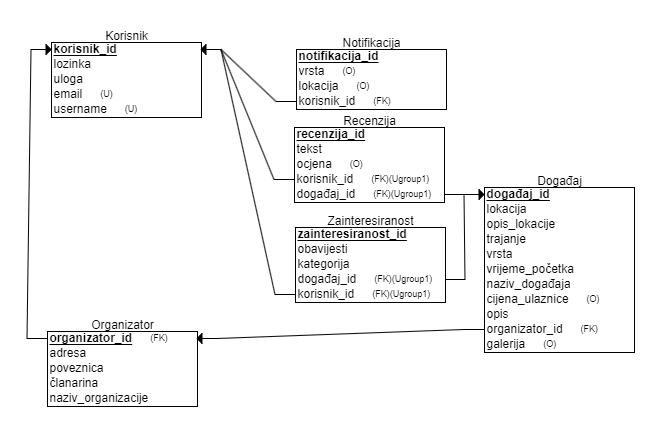
\includegraphics[scale=0.9]{slike/baza.png} %veličina slike u odnosu na originalnu datoteku i pozicija slike
					\centering
					\caption{Dijagram baze podataka}
					\label{fig:promjene}
				\end{figure}
				\eject	
				
			
			
		\section{Dijagram razreda}
		
			Na slikama \textbf{4.3, 4.4, 4.5 i 4.6} su prikazani razredi koji pripadaju \textit{backend} dijelu projekta te oni predstavljaju i odgovaraju stvarnom stanju implementacije sustava te su generirani iz same implementacije. 
			\newline
			\newline
			Razredi prikazani na slici \textbf{4.3} su razredi kontroleri. Ti razredi su ključni dijelovi koji upravljaju pristiglim zahtjevima, određuju rute te obrađuju logiku aplikacije. Obično se koriste za implementaciju HTTP metoda poput \textbf{GET, POST, PUT i DELETE} za obrađivanje zahtjeva koji dolaze od klijenata. Razredi koji imaju svoje kontrolere su \textbf{Korisnik, Organizator,  Događaj, Notifikacija i Transakcije}. Na primjeru KorisnikControllera ćemo detaljnije opisati metode i članske varijable koje su korištene za spajanje sa servisnim slojem.
			\newline
			
			\textbf{KorisnikController} ima metode: 
			\begin{itemize}
				\item getAll - vraća listu Korisnika
				\item delete - kao argument prima ID Korisnika te ga briše ukoliko postoji
				\item validate - prima Korisnika te vraća ResponseEntity, služi validaciji Korisnika
				\item register - kao argument prima KorsnikDTO, a vraća ResponseEntity koji je string
				\item update - služi promjeni i ažuriranju podataka Korisnika
			\end{itemize}
			
			Isto ima i članske varijable tipa KorisnikService i OrganizatorServiceJpa  preko kojih se obavlja poslovna logika (operacije nad podacima, pristupanje bazi podataka ili komunikacija s vanjskim servisima).
			\newline

			Razredi prikazani na slici \textbf{4.4} su razredi servisi. Razredi servisi u Spring Bootu predstavljaju komponente koje sadrže poslovnu logiku aplikacije, pristupaju podacima i obavljaju operacije koje nisu specifične za obradu HTTP zahtjeva. Oni često služe kao posrednici između kontrolera i sloja pristupa podacima (Repository sloj) te obavljaju ključne funkcije za obradu podataka, poslovnu logiku i vanjske integracije. U našem primjeru ostvarili smo prvo sučelja koja smo zatim implementirali.
			Razredi koji imaju svoje servise su \textbf{Korisnik, Organizator, Događaj, Notifikacija, Zainteresiranost, EmailSender, Misc i Recenzija}. Na primjeru KorisnikSerivce ćemo detaljnije opisati metode i članske varijable.
			\newline
			
			\textbf{KorisnikService} sučelje ima metode: 
			\begin{itemize}
				\item listAll - vraća listu Korisnika
				\item findById - prima id kao argument, a ako postoji Korisnik s tim id, njega vraća
				\item findByUsername - prima username kao argument, a ako postoji korisnik s tim usernamom njega vraća
				\item findByEmail - prima email kao argument, a ako postoji korisnik s tim emailom njega vraća
				\item registerUser - kao argument prima KorsnikDTO, a boolean ovisno o uspješnosti
				\item updateUser - kao argument prima KorsnikDTO i ID Korisnika, a boolean ovisno o uspješnosti
				\item deleteUser - kao argument prima Korisnika i briše ga ukoliko postoji
			\end{itemize}
			
			Implementacija sučelja KorisnikService, KorisnikServiceJpa, isto ima i članske varijable tipa KorisnikRepository i PasswordEncoder. Razred repozitorija u Spring Bootu predstavlja sloj pristupa podacima (data access layer) i obično se koristi za komunikaciju s bazom podataka. Ovi repozitoriji pružaju apstrakciju za operacije nad podacima, kao što su dohvaćanje, spremanje, ažuriranje ili brisanje podataka. Instanca PasswordEncoder služi nam za registraciju korisnika te za ažuriranje njegovih podataka kada dolazi do promjene lozinke.
			\newline

			\eject
			Razredi prikazani na slici 4.5. su razredi modeli. Struktura baze podataka u aplikaciji odražava se upravo model razredima; osim što imaju svoje pripadne atributa, razredi također implementiraju metode koje ostvaruju interakciju s bazom podataka. \\ 
			\\ Razred Korisnik reprezentira općeg korisnika aplikacije. Specificira ga atribut "uloga" koja određuje je li korisnik administrator, posjetitelj ili organizator.
			\\ Razred Organizator reprezentira korisnika s organizatorskim računom. Organizatori mogu pregledavati svoje postojeće događaje i postavljati nove događaje.
			\\ Razred Recenzija reprezentira korisnikov osvrt na događaj u obliku ocjene i komentara.
			\\ Razred Notifikacija reprezentira obavijest koja se šalje korisniku. Korisnik ima mogućnost uključiti notifikacije za određenu vrstu događaja te za lokaciju na kojoj se događaji organiziraju.
			\\ Razred Zainteresiranost reprezentira korisnikovu interakciju s postavljenim događajima. Korisnikova zainteresiranost ima tri razine: "sigurno dolazim", "možda dolazim", "ne dolazim".
			\\ Razred Dogadaj reprezentira događaj koji je postavio organizator. Lokacija događaja predstavljena je gradskom četvrti - kvartom.
			\\ Razred Misc skraćeno od ”miscellaneous”, ovaj razred služi za spremanje globalnih postavki aplikacija u obliku ključ-vrijednost. Sadrži atribute ime i vrijednost.
			Osim navedenih razreda na slici su također prikazane enumeracije: 
					Kategorija - kategorija zainteresiranosti korisnika za događaj,
					Kvartovi - kvartovi grada Zagreba gdje se organiziraju događaji,
					Uloga - uloga korisnika i 
					Vrste - različite vrste događaja
			
			\pagebreak
			
			\begin{figure}[H]
				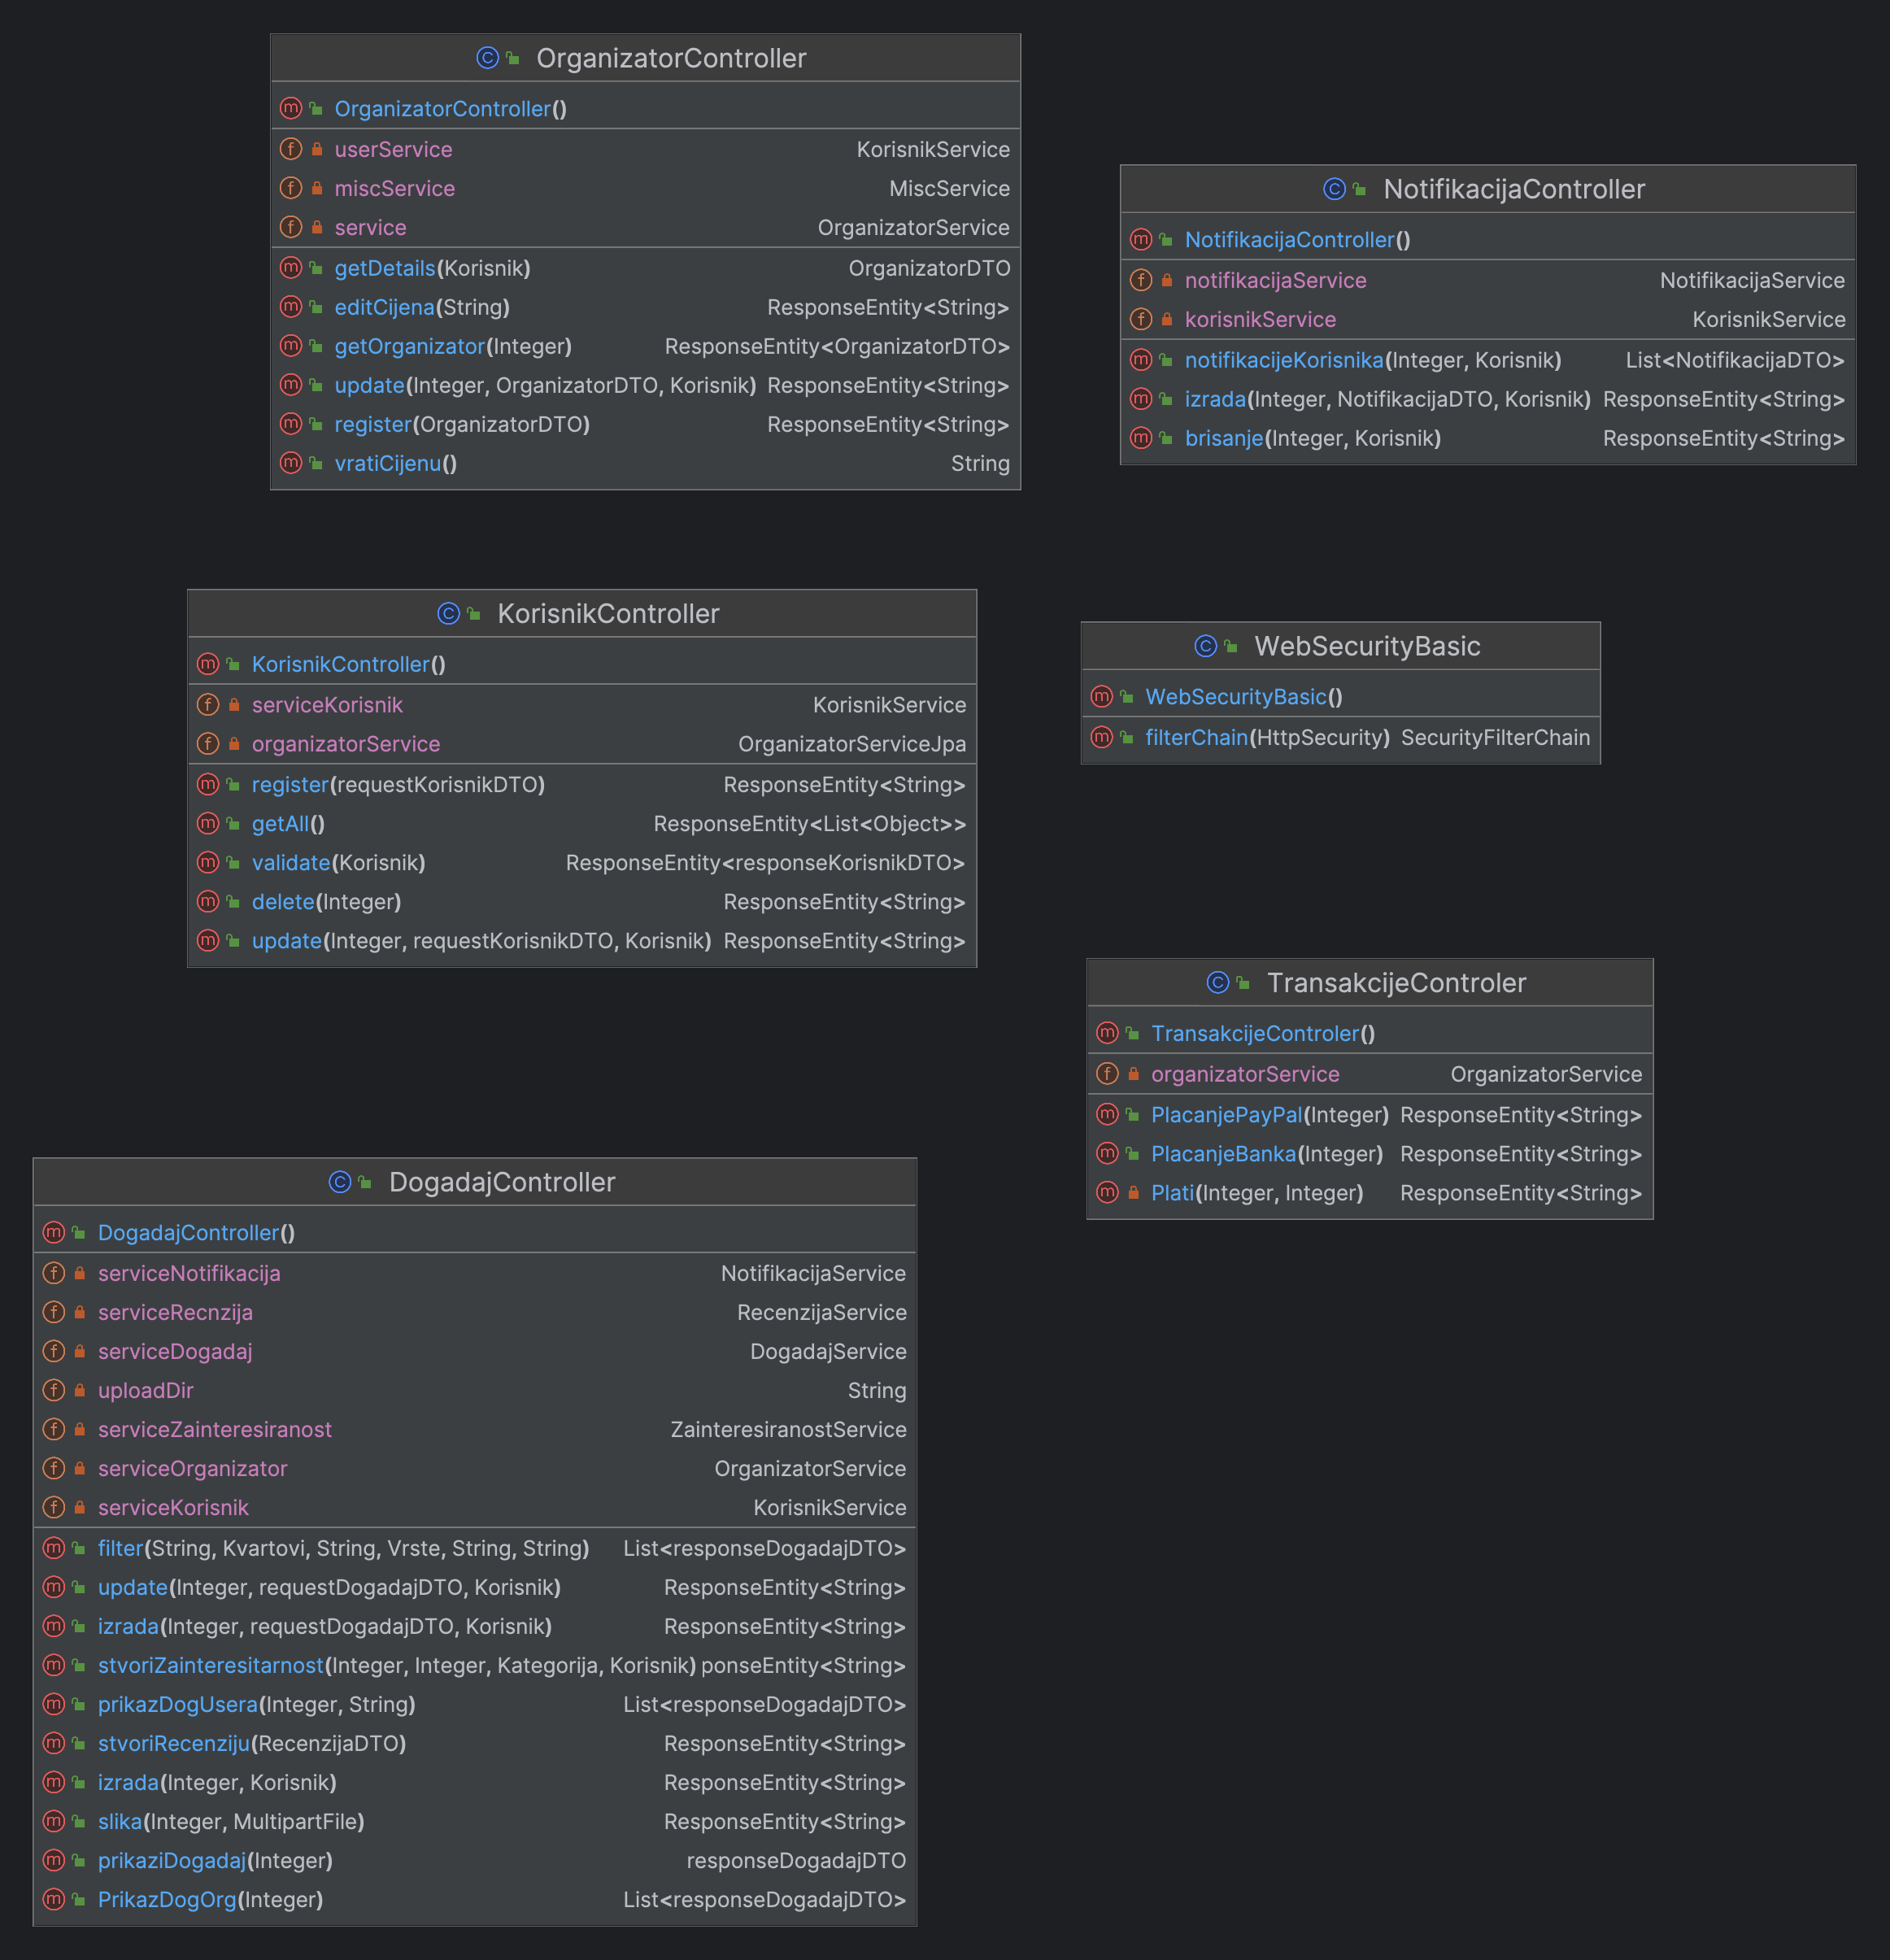
\includegraphics[scale=0.2]{dijagramiKlasa/kontroleri.png} %veličina slike u odnosu na originalnu datoteku i pozicija slike
				\centering
				\caption{Dijagram razreda - Kontroleri}
				\label{fig:promjene}
			\end{figure}
			
			\begin{figure}[H]
				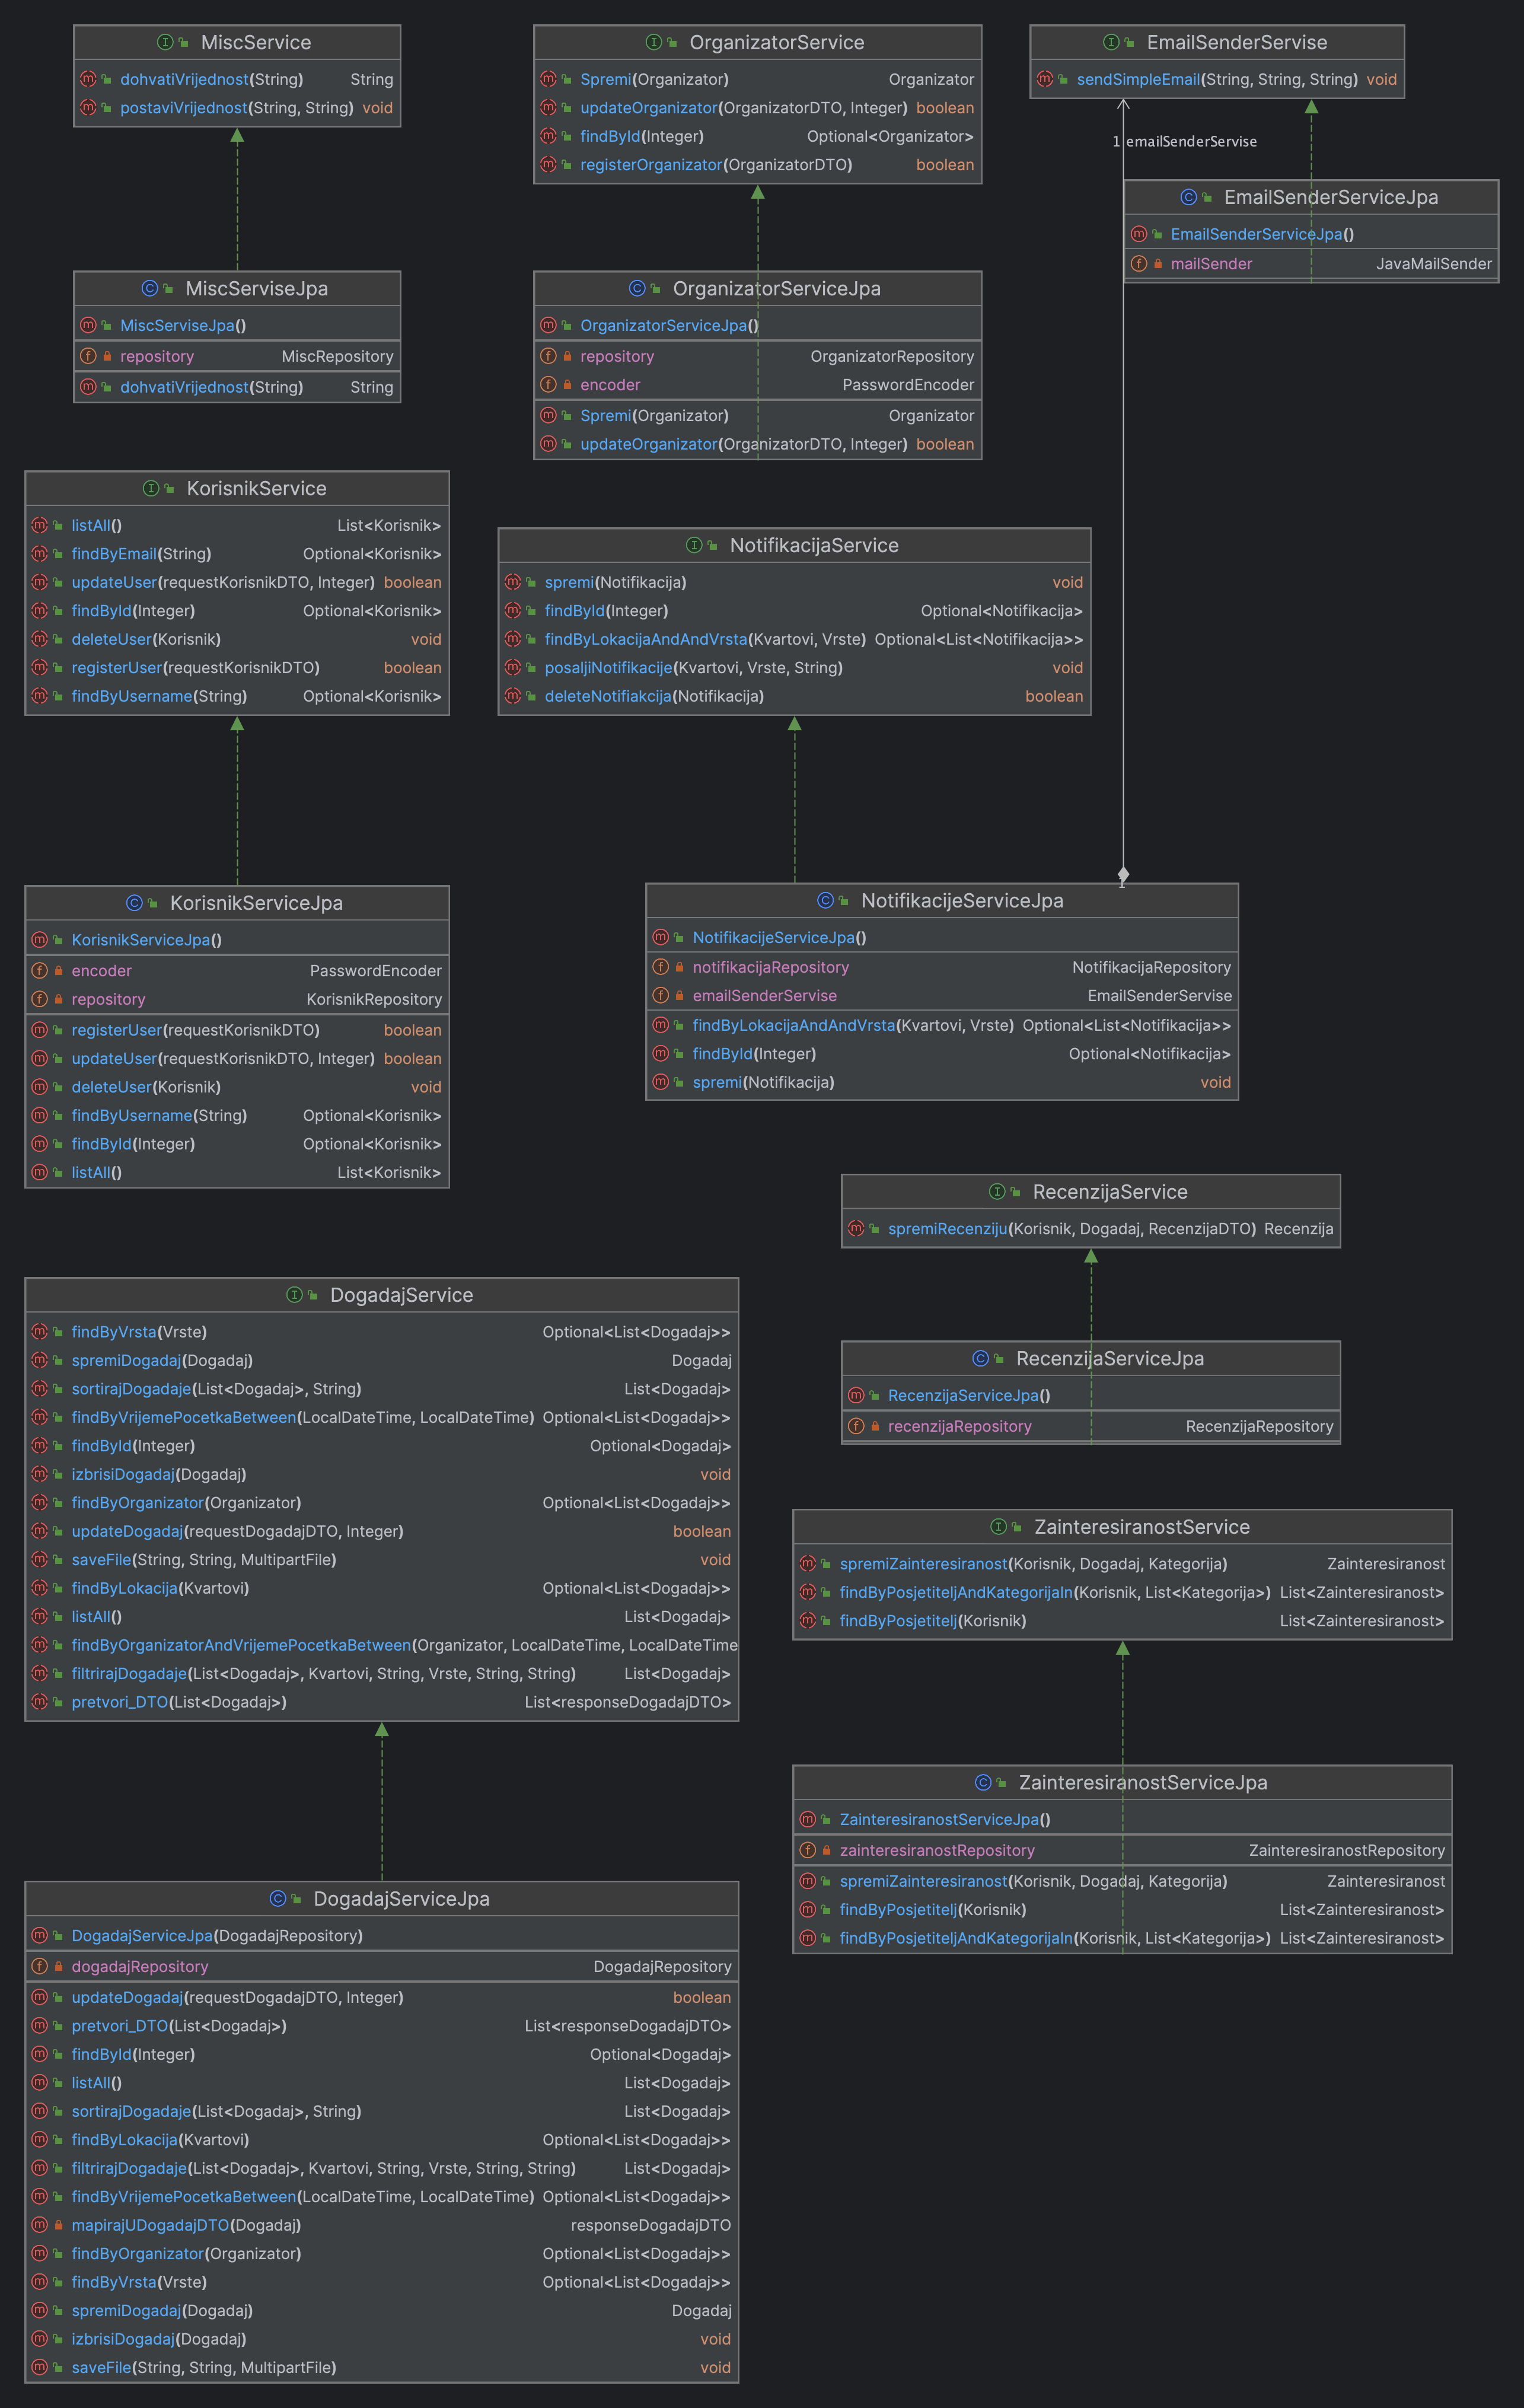
\includegraphics[scale=0.13]{dijagramiKlasa/servisi.png} %veličina slike u odnosu na originalnu datoteku i pozicija slike
				\centering
				\caption{Dijagram razreda - Servisi}
				\label{fig:promjene}
			\end{figure}
			
			\begin{figure}[H]
				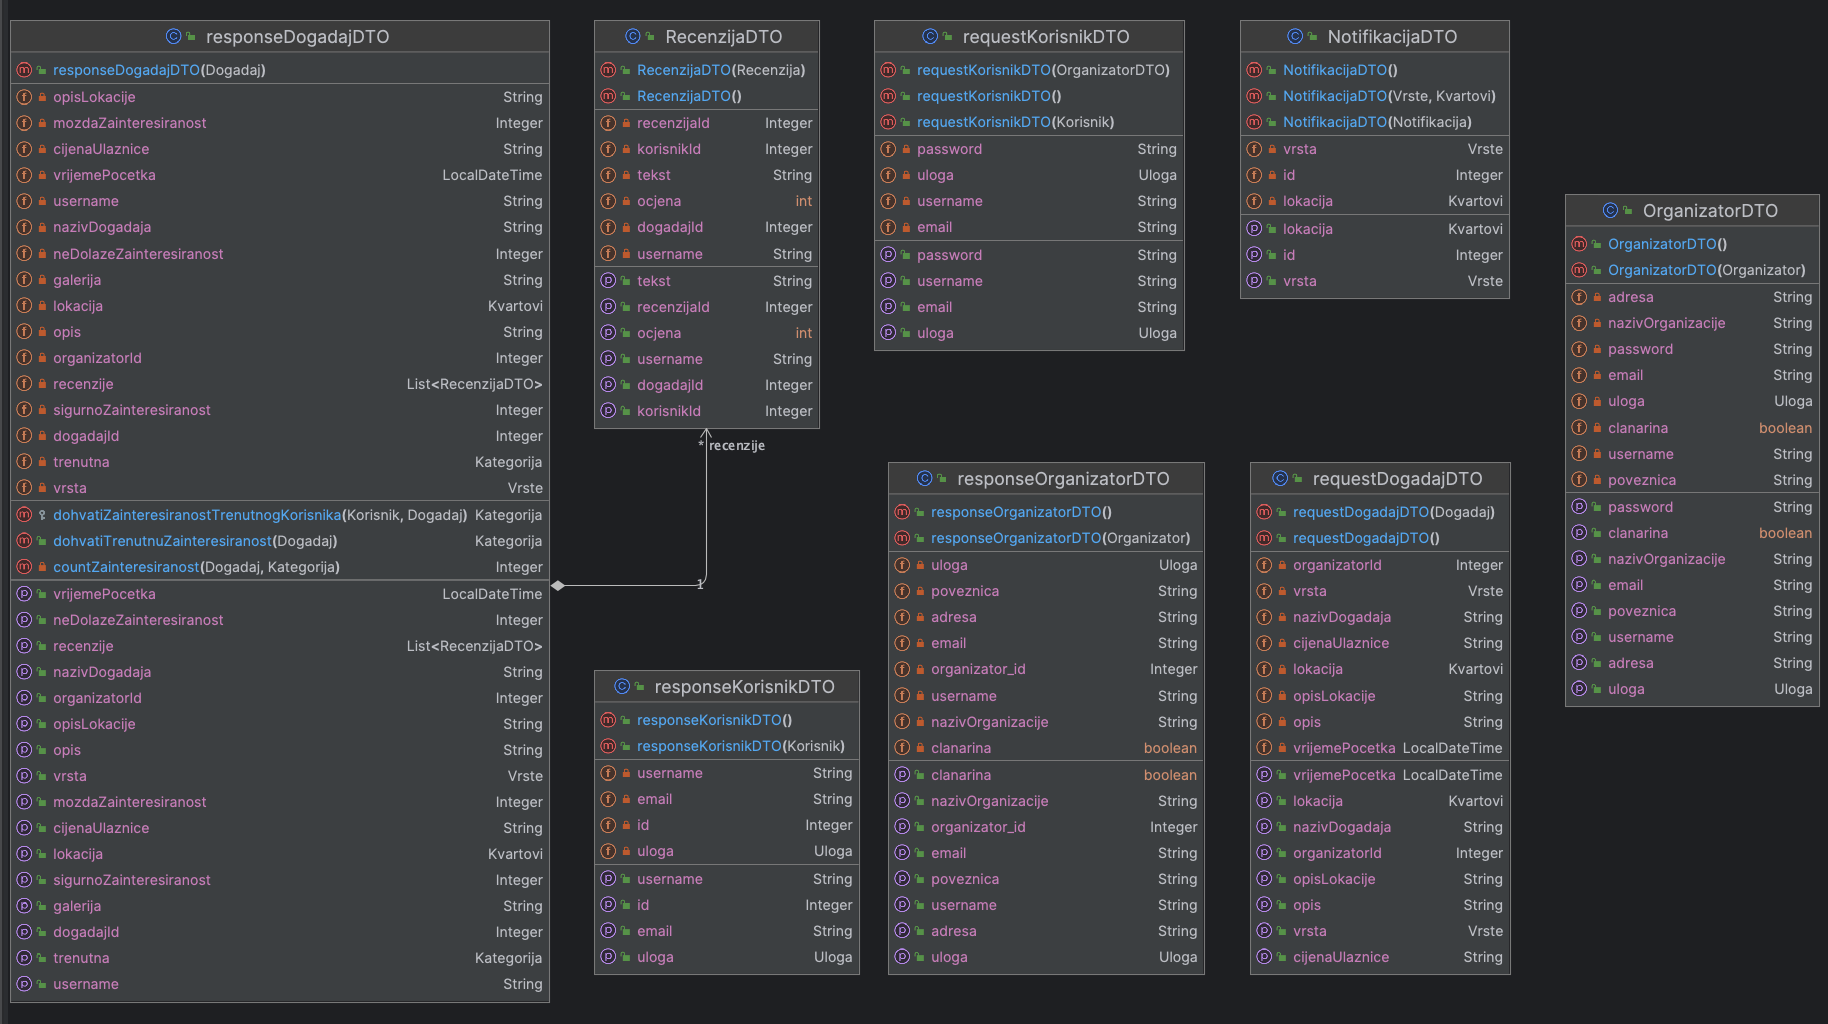
\includegraphics[scale=0.5]{dijagramiKlasa/dtos.png} %veličina slike u odnosu na originalnu datoteku i pozicija slike
				\centering
				\caption{Dijagram razreda - Data Transfer Objects}
				\label{fig:promjene}
			\end{figure}
			
			
			\begin{figure}[H]
				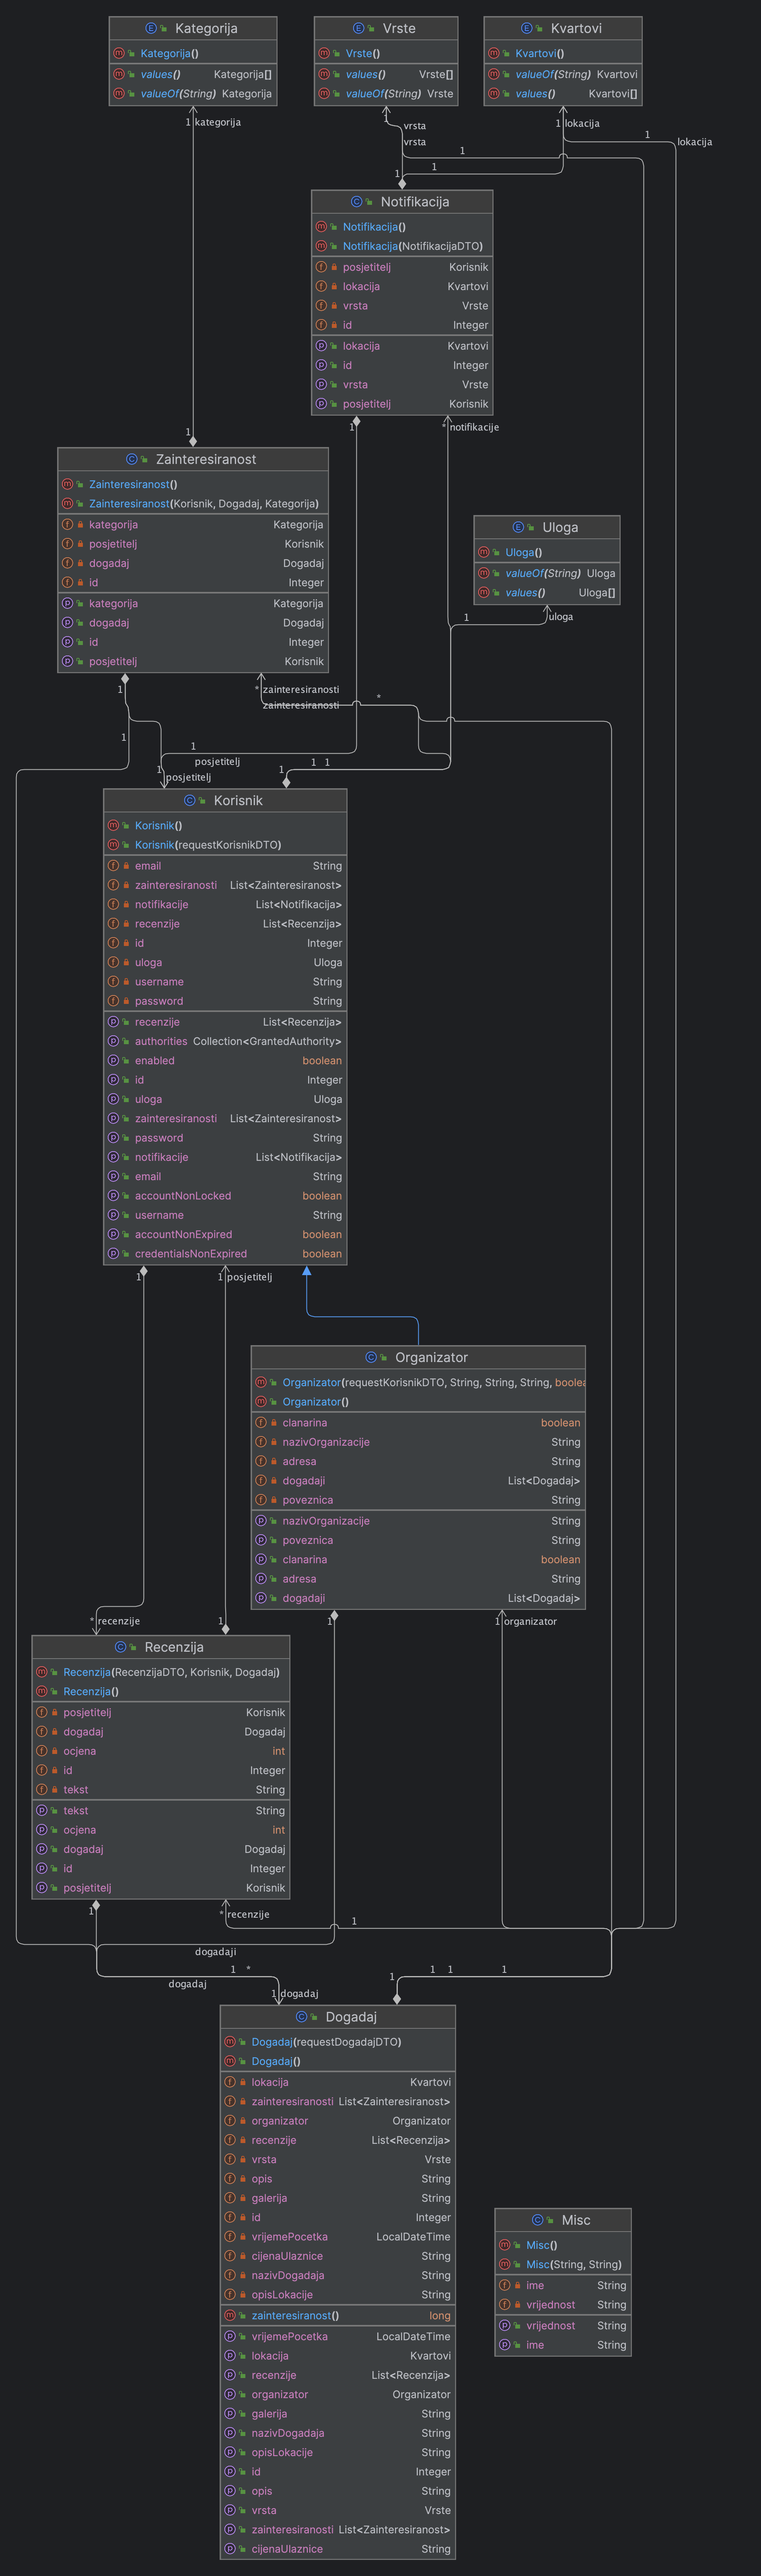
\includegraphics[scale=0.1]{dijagramiKlasa/models.png} %veličina slike u odnosu na originalnu datoteku i pozicija slike
				\centering
				\caption{Dijagram razreda - Models}
				\label{fig:promjene}
			\end{figure}
			
			
			\eject
		
		\section{Dijagram stanja}
			
			
			Dijagram stanja opisuje dinamičko ponašanje dijela sustava u vremenu; prikazuje stanja objekta i prijelaze iz jednog stanja u drugo temeljene na događajima. Na slici 4.7 prikazan je dijagram stanja za korisnika - posjetitelja. Kada se korisnik prijavi prikazuje mu se početna stranica na kojoj su vidljivi događaji, filter pomoću kojeg može odlučiti koje događaje želi pregledati, te navigacijska traka preko kojeg pristupa svim događajima, događajima za koje je označio "Sigurno dolazim" ili "Možda dolazim" te profilu. Klikom na "Moji događaji" prikazuju mu se događaji na koje je prethodno reagirao sa "Sigurno dolazim" ili "Možda dolazim". Ako među ovim događajima postoje događaji koji su završili i nije prošlo 48 sati od njihovog završetka, korisnik za njih može izraditi recenziju. Klikom na korisničko ime - profil prikazuje mu se stranica profila na kojoj može promijeniti osobne podatke te urediti postavke pretplata na obavijesti.
			
			\begin{figure}[H]
			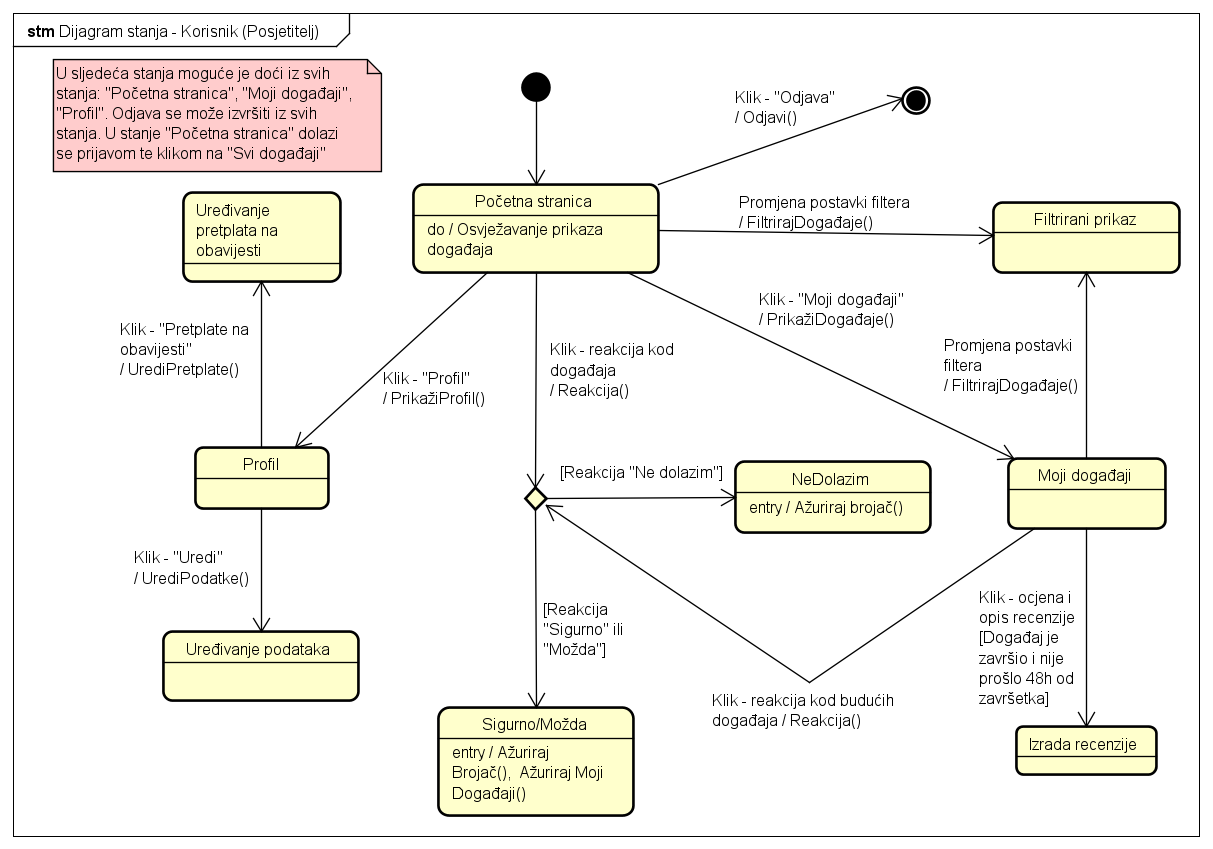
\includegraphics[scale=0.50]{dijagrami/DijagramStanja-Korisnik.png}
			\centering
			\caption{Dijagram stanja - Korisnik (Posjetitelj)}
			\label{fig:promjene}
			\end{figure}
			
			\eject 
		
		\section{Dijagram aktivnosti}
			
			Dijagram aktivnosti primjenjuje se za modeliranje poslovnih procesa, upravljačkog i podatkovnog toka. Na slici 4.8 prikazan je dijagram aktivnosti za proces stvaranje novog događaja. Nakon prijave organizator na početnoj stranici odabire opciju postavljanja događaja. Otvara mu se stranica za postavljanje događaja na kojoj unosi sve potrebne podatke o događaju. Ako organizator želi događaj bez plaćanja ulaza, podaci o događaju se odmah procesiraju, spremaju u bazu te se organizatoru prikazuje potvrda o uspješno postavljenom događaju. Ako organizator želi događaj koji će imati plaćanje ulaza, provodi se provjera članarine. Ako je članarina plaćena, proces se nastavlja jednako kao i u slučaju besplatnog događaja. Ako nije, aplikacija obavješta organizatora da članarina nije plaćena te organizator ima dvije mogućnosti: ponovno unijeti podatke o događaju i početi proces postavljanja ispočetka ili odustati od postavljanja događaja.
			
			\begin{figure}[H]
				\includegraphics[scale=0.48]{dijagrami/DijagramAktivnosti-Postavljanje_događaja.png}
				\centering
				\caption{Dijagram aktivnosti - Postavljanje događaja (Organizator)}
				\label{fig:promjene}
			\end{figure}
			
			\eject
		\section{Dijagram komponenti}
		
		Dijagram komponenti na slici opisuje organizaciju, međuovisnost komponenti i odnose prema okolini - prikazuje komponente aplikacije i glavna korištena sučelja. Web aplikacija Korisnik pristupa aplikaciji koristeći web preglednik te preko sučelja za dohvaćanje HTML-a, CSS i JS-a poslužuje mu se frontend dio aplikacije. Pomoću REST API sučelja komunicira te mu se poslužuju podaci povezani s backend dijelom. Svaka od opisanih komponenti može imati ovisnosti prema drugim resursima, tako je backend dio povezan sa bazom podataka korištenjem Jakarta Persistance API - JPA. 
		Web aplikacija Eventio prati MVC arhitekturu te stoga postoji distinkcija između frontend i backend dijela aplikacje što je vidljivo i na ovom dijagramu. "View" dio arhitekture je frontend u kojem koristimo React library koji nam omogućuje podijelu na više komponenata te se brine o njihovom spajanju. App.jsx komponenta web aplikacije brine o prijavi korisnika te ovisno o ulozi korisnika Router prikazuje potrebne komponente. Također su prikazane komponente backend sloja, redom: Kontroleri, Servisi i Repozitoriji. Predstavljaju "Model" i "Controller" dio MVC arhitekture te je u dijagramu prikazana njihova međuovisnost.
				
		\begin{figure}[H]
			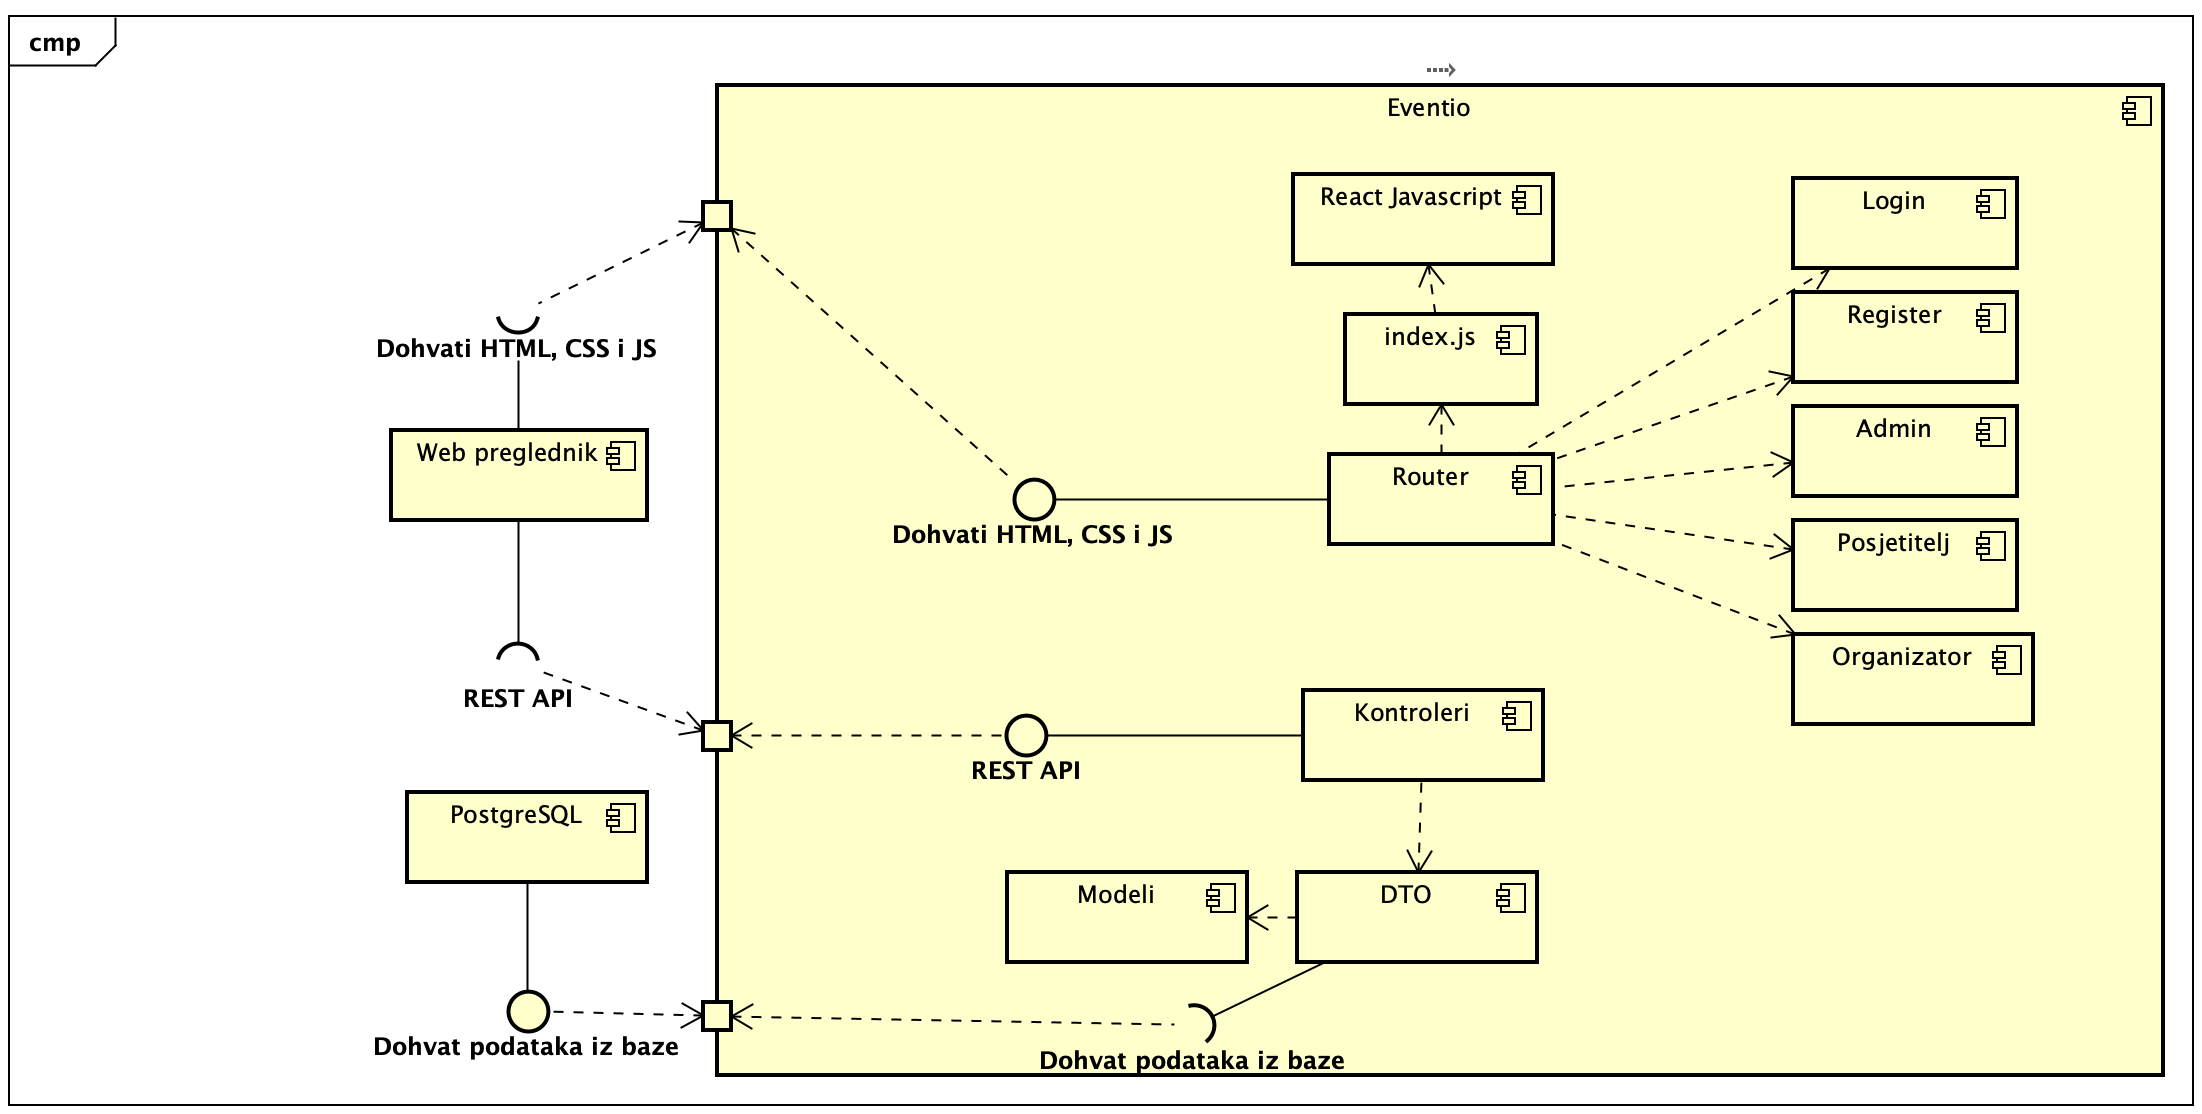
\includegraphics[scale=0.48]{dijagrami/DijagramKomponenti.png}
			\centering
			\caption{Dijagram komponenti}
			\label{fig:promjene}
		\end{figure}